\documentclass[17pt]{article}

\usepackage[margin=1in, paperwidth=8.5in, paperheight=11in]{geometry}
\usepackage{amsmath}
\usepackage[document]{ragged2e}
\usepackage{graphicx}
\usepackage{listings}
\usepackage{color}

\definecolor{dkgreen}{rgb}{0,0.6,0}
\definecolor{gray}{rgb}{0.5,0.5,0.5}
\definecolor{mauve}{rgb}{0.58,0,0.82}

\lstset{frame=tb,
  language=Python,
  aboveskip=3mm,
  belowskip=3mm,
  showstringspaces=false,
  columns=flexible,
  basicstyle={\small\ttfamily},
  numbers=none,
  numberstyle=\tiny\color{gray},
  keywordstyle=\color{blue},
  commentstyle=\color{dkgreen},
  stringstyle=\color{mauve},
  breaklines=true,
  breakatwhitespace=true,
  tabsize=3
}

\begin{document}

\title{\textbf{Generalized linear model: Bioassay with importance sampling}}
\maketitle

\section{Calculate posterior density in a grid around the prior $ \alpha: 0 \pm 4, \beta: 10 \pm 20 $ and plot a heatmap of the density}

$$ n = np.array([5, 5, 5, 5]) $$
$$ x = np.array([-0.86, -0.30, -0.05, 0.73]) $$
$$ y = np.array([0, 1, 3, 5]) $$
$$ p = 0.5 $$
$$ sigma\_a = 2 $$
$$ sigma\_b = 10 $$
$$ mu\_a = 0 $$
$$ mu\_b = 10 $$
$$ mean = [0, 10] $$

The covariance is calculated the following way:
$$ \mathbf{covariance = np.array([sigma\_a^2, p * sigma\_a, sigma\_b], [p * sigma\_a * sigma\_b, siga\_b^2])} $$

The prior is calculated with the following function:
$$ \mathbf{prior = stats.multivariate\_normal(mean, covariance)} $$

The density distribution for the prior is calculated with this function:
$$ \mathbf{prior\_density\_dist = prior.pdf(grid)} $$

\begin{center}
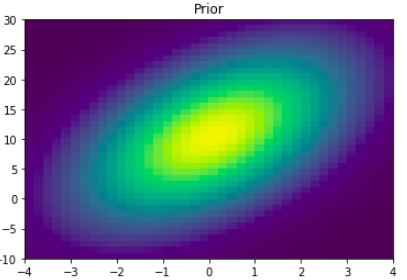
\includegraphics[width=10cm, height=5cm]{prior.png}
\end{center} 

For calculating the likelihood, I am using the function \textbf{bioassaylp} that was provided for us in the examples. Alternatively, the equation (3.15) from the book can be used to calculate the likelihood. \\
The posterior is the calculated the following way:
$$ \mathbf{posterior = np.exp(likelihood) * prior\_density\_dist} $$
Alternatively, we can use the equation (3.16) from the book.
\begin{center}
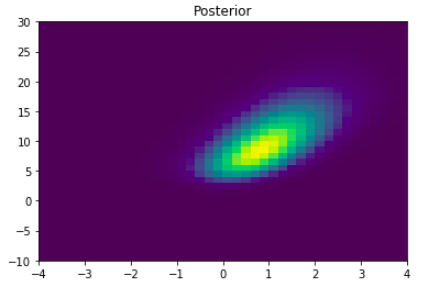
\includegraphics[width=10cm, height=5cm]{posterior.png}
\end{center}


\section{Sample draws of $ \alpha $ and $ \beta $ from the prior distribution} 
We draw 5000 samples from the prior distribution the following way:
$$ \mathbf{S = 5000} $$
$$ \mathbf{random\_samples = prior.rvs(S)} $$


\section{Compute the importance ratios for each draw (target distribution is the posterior)}
We get $\alpha$ and $\beta$ from the random samples that we have drawn.

Then we calculate the weights with the same \textbf{bioassaylp} that was provided for us in the examples. Alternatively, we can use the equation (10.3) from the book to calculate the weights.

Then we normalize the weights this way:
$$ \mathbf{weights\_norm = \frac{weights}{np.sum(weights)}} $$


\section{Using the importance ratios, compute the effective sample size $\mathbf{S_{eff}}$ and report it}

The effective sample size is cauculated with the following formula:
$$ \mathbf{S_{eff} = \frac{1}{\sum_{s=1}^S(w(\theta))^2}} $$

\textbf{The value of $ \mathbf{S_{eff}}$ is: 1347.1803}


\section{Compute the posterior mean using the importance sampling and report it}

The posterior mean is calculated the following way:
$$ \mathbf{mean\_posterior = sum(weights[:,None] * random\_samples) / sum(weights)} $$

\textbf{The posterior $\mathbf{\alpha}$ mean is: 0.9710}

\textbf{The posterior $\mathbf{\beta}$ mean is: 10.5057}


\section{Use importance resampling to obtain a posterior sample size 1000 of $\mathbf{\alpha}$ and $\mathbf{\beta}$}

We obtain the posterior sample the following way:
$$ \mathbf{sampling = np.random.choice(a=S, size=1000, replace=False, p=weights\_norm)} $$
$$ \mathbf{posterior\_sample = random\_samples[sampling]} $$
Alternatively, we can use the steps explained in the book (page 266).

\textbf{The posterior resampled $\mathbf{\alpha}$ mean is: 1.0292}

\textbf{The posterior resampled $\mathbf{\beta}$ mean is: 11.2210}


\section{Using the posterior sample obtained via importance sampling}
\subsection{Plot a scatterplot of the obtained posterior sample and compare that to the heatmap plotted earlier}
\subsection{Report an estimate for $\mathbf{p(\beta>0|x,n,y|)}$, that is, the probability that that drug is harmful.}
\subsection{Draw a histogram of the draws from the posterior distribution of the LD50 conditional on $\mathbf{\beta>0}$}

\begin{center}
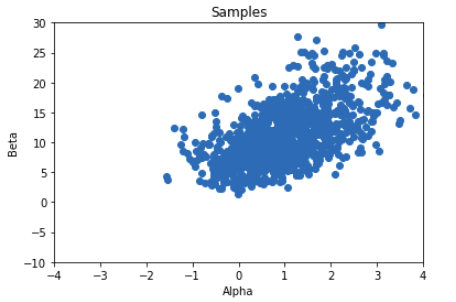
\includegraphics[width=10cm, height=5cm]{scatter_posterior_samples.png}
\end{center}

\begin{center}
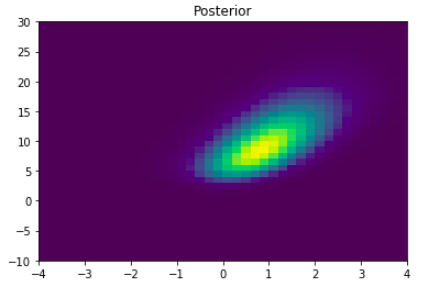
\includegraphics[width=10cm, height=5cm]{posterior.png}
\end{center}

The probability that the drug is harmful is calculated this way:
$$ \mathbf{b_idx = beta>0} $$
$$ \mathbf{prob = (beta[b_idx].size / beta.size)} $$

\textbf{The probability that the drug is harmful is: 1.0}

We can see that from 1000 drawn samples the probability is 100 \% that the drug is harmful but this doesn't mean that it will that way for every single sample. So, we can say the the probability that the drug is harmful is: 0.99999.

We compute the LD50 with the following equation for 1000 samples:
$$ \mathbf{ld50 = \frac{-\alpha}{\beta}} $$

\begin{center}
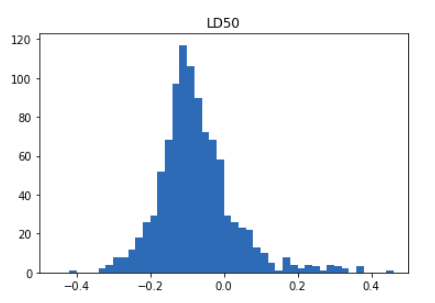
\includegraphics[width=10cm, height=5cm]{ld50.png}
\end{center}

\newpage

\begin{align}
\textbf{SOURCE CODE}
\end{align}

\begin{lstlisting}
import numpy as np
import scipy.stats as stats
from scipy.special import expit
import matplotlib.pyplot as plt

def bioassaylp(a, b, x, y, n):
    a = np.expand_dims(a, axis=-1)
    b = np.expand_dims(b, axis=-1)
    # these help using chain rule in derivation
    t = a + b*x
    et = np.exp(t)
    z = et/(1.+et)
    # negative log posterior (error function to be minimized)
    lp = np.sum(y*np.log(z)+ (n-y)*np.log(1.0-z), axis=-1)
    return lp
    
n = np.array([5, 5, 5, 5])
x = np.array([-0.86, -0.30, -0.05, 0.73])
y = np.array([0, 1, 3, 5])

# mean_alpha_beta = [0, 10]
# cov = np.matrix("4, 10; 10, 100")
corr = 0.5
sigma_a = 2
sigma_b = 10
mu_a = 0
mu_b = 10
p = 0.5


mean = np.array([mu_a,mu_b])
covariance = np.array([[sigma_a**2,p*sigma_a*sigma_b],[p*sigma_a*sigma_b,sigma_b**2]])
prior = stats.multivariate_normal(mean, covariance)

alpha = np.transpose(np.arange(-4, 4, 0.2))
beta = np.transpose(np.arange(-10, 30, 1))

alpha, beta = np.meshgrid(alpha, beta)
grid = np.dstack((alpha, beta))

prior_density_dist = prior.pdf(grid)

plt.imshow(
    prior_density_dist,
    origin = 'lower',
    aspect = 'auto',
    extent = (-4, 4, -10, 30)
)
plt.title('Prior')
plt.show()

likelihood = bioassaylp(alpha, beta, x, y, n)
posterior = np.exp(likelihood) * prior_density_dist

plt.imshow(
    posterior,
    origin = 'lower',
    aspect = 'auto',
    extent = (-4, 4, -10, 30)
)
plt.title('Posterior')
plt.show()


# b)
S = 5000
random_samples = prior.rvs(S)


def bioassaylp_modified(a, b, x, y, n):
    a = np.expand_dims(a, axis=-1)
    b = np.expand_dims(b, axis=-1)
    # these help using chain rule in derivation
    t = a + b*x
    et = np.exp(t)
    z = et/(1.+et)
    for i in range(len(z)):
        for j in range(len(z[i])):
            if z[i][j] == 1:
                z[i][j] -= 1e-12
            if np.any(np.absolute(z[i][j]) < 1e-12):
                z[i][j] = 1e-12
    # negative log posterior (error function to be minimized)
    lp = np.sum(y*np.log(z)+ (n-y)*np.log(1.0-z), axis=-1)
    return lp
    
    
    
# c)
alpha_random = []
beta_random = []
for i in range(len(random_samples)):
    alpha_random.append(random_samples[i][0])
    beta_random.append(random_samples[i][1])

    
weights = bioassaylp_modified(alpha_random, beta_random, x, y, n)
weights = np.array(np.exp(weights))
weights_norm = (weights)/np.sum(weights)
s_eff = 1 / np.sum(weights_norm ** 2)
print('The value of S_eff is {0}'.format(s_eff))
mean_posterior = sum(weights[:,None] * random_samples) / sum(weights)
print('Posterior alpha mean is: {0}'.format(mean_posterior[0]))
print('Posterior beta mean is: {0}'.format(mean_posterior[1]))



sampling = np.random.choice(a=S, size=1000, replace=False, p=weights_norm)
posterior_sample = random_samples[sampling]

alpha = posterior_sample[:,0]
beta = posterior_sample[:,1]

print('Mean of resampled alpha: {0}'.format(np.mean(alpha)))
print('Mean of resampled beta: {0}'.format(np.mean(beta)))


plt.scatter(alpha, beta)
plt.xlim(-4, 4)
plt.ylim(-10, 30)
plt.xlabel('Alpha')
plt.ylabel('Beta')
plt.title('Samples')
plt.show()

plt.imshow(
    prior_density_dist,
    origin = 'lower',
    aspect = 'auto',
    extent = (-4, 4, -10, 30)
)
plt.title('Posterior')


b_idx = beta>0
prob = (beta[b_idx].size / beta.size)
print("The probability that the drug if harmful is: {0}".format(prob))


ld50 = -alpha[b_pos] / beta[b_pos]
plt.hist(ld50, np.arange(-50, 50, 0.02))
plt.xlim(-0.5, 0.5)
plt.title('LD50')

\end{lstlisting}


\end{document}





